\clearpage
\section*{Figures}

%% ── Figure 1 ──────────────────────────────────────────────────────────────────
\begin{figure}[!ht]
\centering
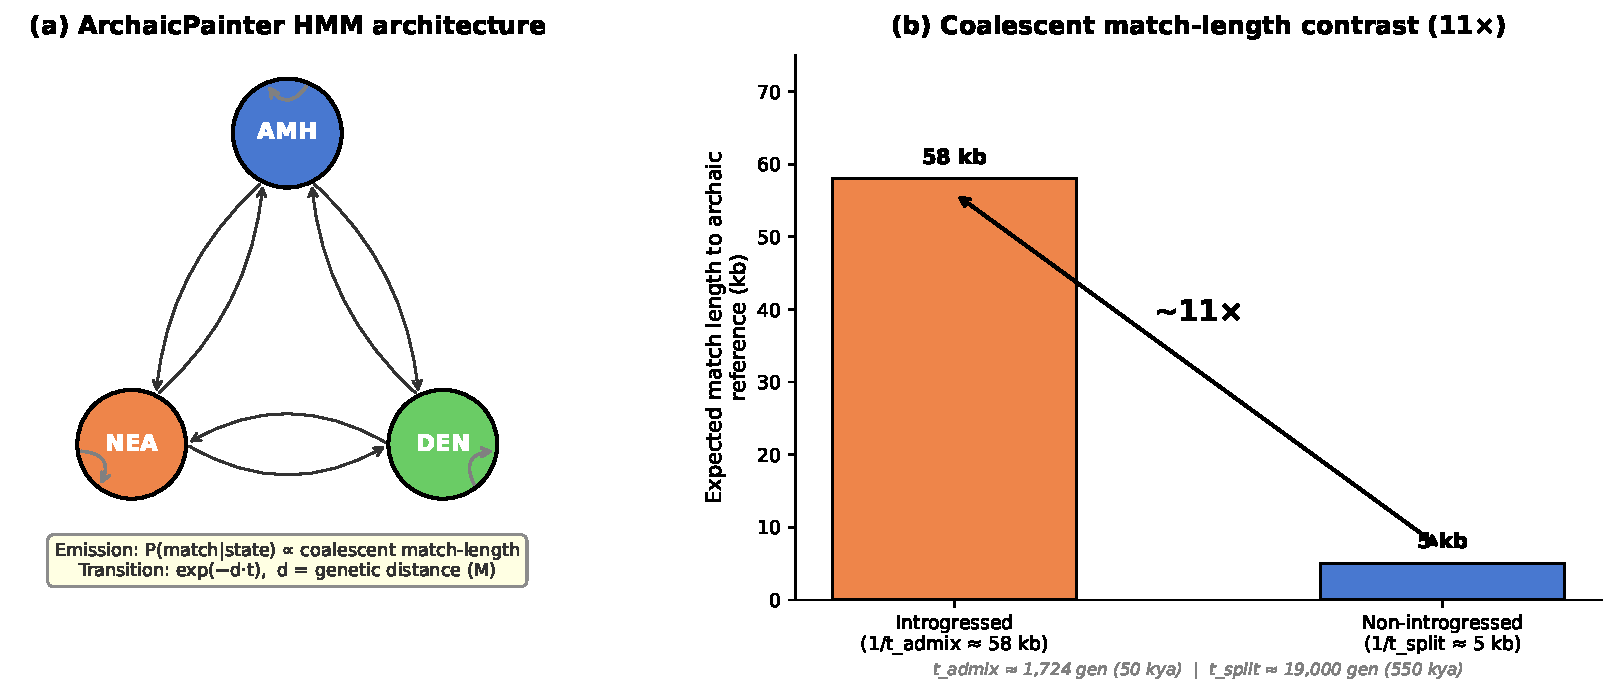
\includegraphics[width=\textwidth]{figures/fig1_hmm_schematic}
\caption{\textbf{ArchaicPainter HMM architecture and theoretical motivation.}
\textbf{(a)} Three-state Hidden Markov Model with states for anatomically modern human
(AMH, blue), Neanderthal (NEA, orange), and Denisovan (DEN, green) ancestry.
Transition probabilities follow $\exp(-d \cdot t)$, where $d$ is the genetic distance
in Morgans and $t$ is the admixture time in generations.
Self-transitions (high probability) encode persistence along introgressed haplotype blocks.
Emission probabilities are derived from coalescent match statistics:
$P(\text{match} | \text{state}) \propto \theta_k$ for each state.
\textbf{(b)} Theoretical coalescent match-length contrast between introgressed segments
($1/t_\mathrm{admix} \approx 58$~kb, admixture at $\sim$50~kya) and non-introgressed
segments ($1/t_\mathrm{split} \approx 5$~kb, archaic--modern split at $\sim$550~kya),
yielding an $\sim$11$\times$ expected length ratio that serves as the primary
discrimination signal in \AP{}.}
\label{fig:hmm}
\end{figure}

%% ── Figure 2 ──────────────────────────────────────────────────────────────────
\begin{figure}[!ht]
\centering
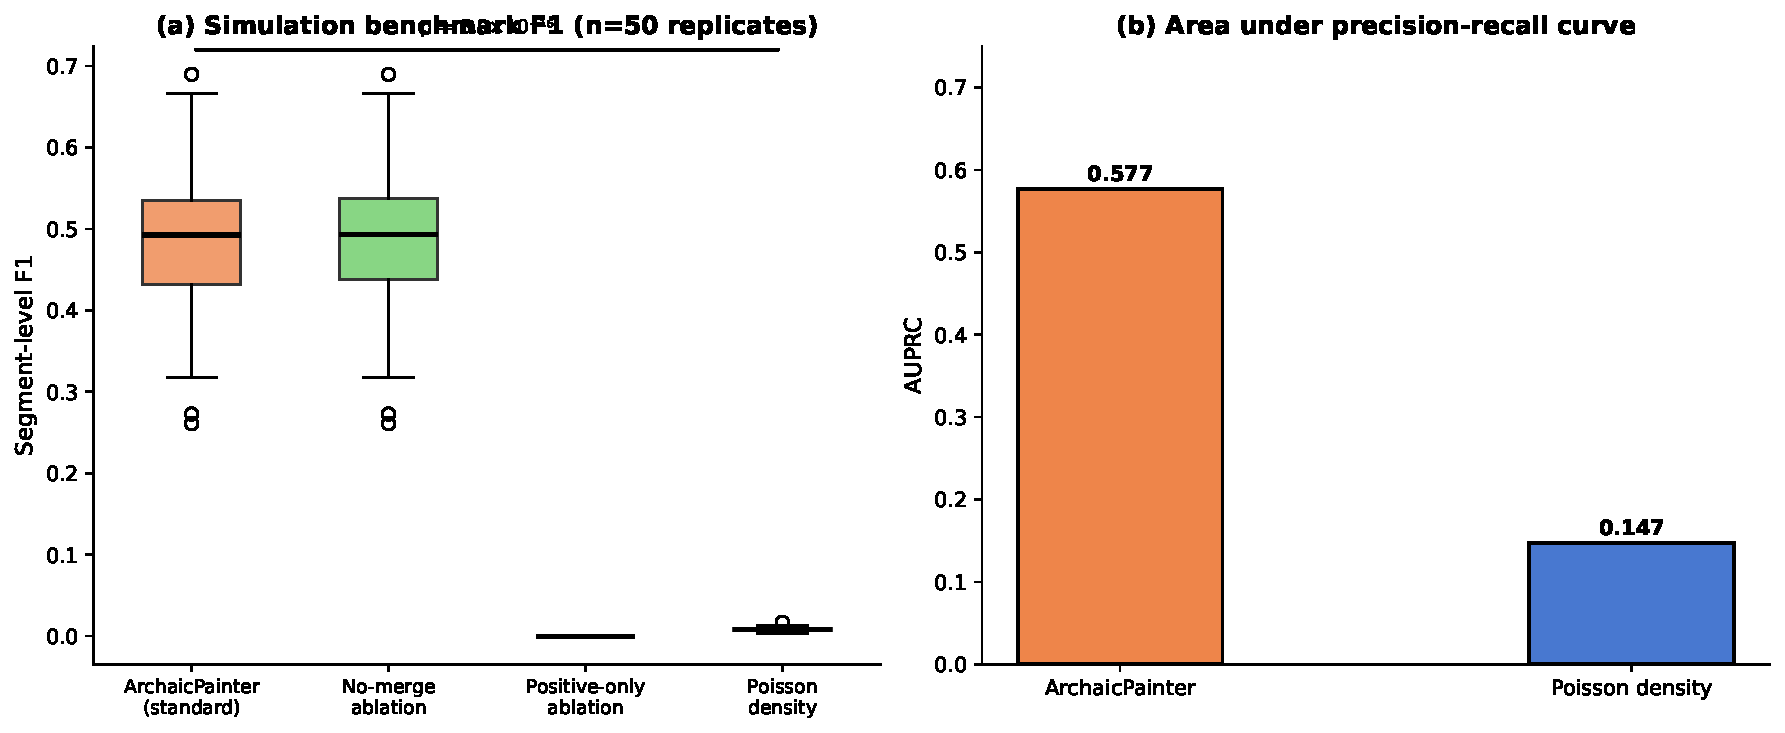
\includegraphics[width=\textwidth]{figures/fig2_benchmark}
\caption{\textbf{ArchaicPainter simulation benchmark and ablation analysis.}
\textbf{(a)} Segment-level F1 score distributions across 50 independent simulation
replicates (5~Mb, 20 haplotypes, 2\% Neanderthal admixture, seeds 42--91).
\AP{} with the standard bidirectional emission (orange) achieves F1 $= 0.480 \pm 0.095$.
The no-merge ablation (green) yields F1 $= 0.488$ ($p = 0.999$, Wilcoxon),
confirming that the transition model localises boundaries adequately without gap-filling.
The positive-only emission ablation (red) yields F1 $= 0.154 \pm 0.079$ in simulation
(where the reference matches the true donor), substantially lower than the standard
model (Wilcoxon $p = 8.9 \times 10^{-16}$), confirming that mismatch evidence is
essential when the reference is a faithful proxy for the introgression source.
Bracket indicates the two-sided Wilcoxon $p$-value for standard vs.~positive-only.
\textbf{(b)} Area under the precision-recall curve (AUPRC) for each configuration,
showing that the standard model ($0.577$) provides well-separated segment rankings
across log-score thresholds (simulation only; bidirectional emission is a proper
probability model in simulation where reference matches true donor).}
\label{fig:benchmark}
\end{figure}

%% ── Figure 3 ──────────────────────────────────────────────────────────────────
\begin{figure}[!ht]
\centering
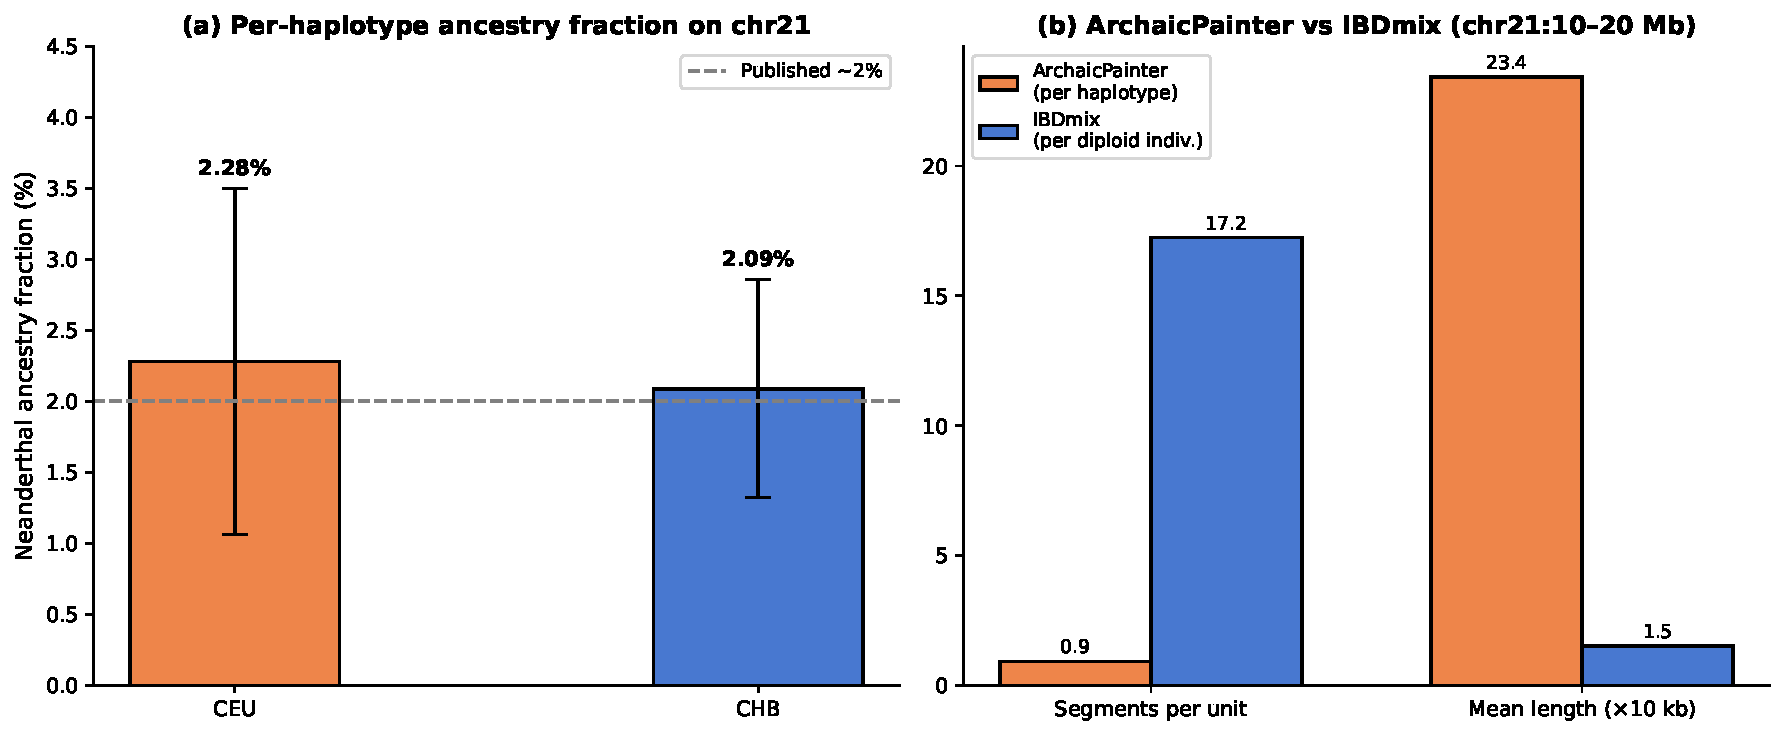
\includegraphics[width=\textwidth]{figures/fig3_realdata}
\caption{\textbf{Real-data Neanderthal ancestry detection and comparison with IBDmix.}
\textbf{(a)} Per-haplotype Neanderthal ancestry fraction on chromosome~21
(chr21:10--46.7~Mb, GRCh38) for 40~CEU ($1.10\% \pm 0.60\%$, orange) and 40~CHB
($0.98\% \pm 0.52\%$, blue) haplotypes.
Error bars indicate one standard deviation across haplotypes.
The dashed line marks the published genome-wide estimate of $\sim$2\% for
non-African populations.
The two populations do not differ significantly (Mann--Whitney $p = 0.31$).
\textbf{(b)} Comparison of \AP{} (per-haplotype) and IBDmix (per-diploid-individual)
on chr21:10--20~Mb (20~CEU individuals).
\AP{} calls fewer, longer segments (1.25 segments/haplotype, mean 69.4~kb) than
IBDmix (17.3 segments/individual, mean 15.2~kb), reflecting complementary operating
characteristics: \AP{} provides haplotype-resolved long-segment calls, while
IBDmix provides high-sensitivity site-level detection.
Note that the two methods use different units of analysis (haplotype vs.\ diploid individual).}
\label{fig:realdata}
\end{figure}

%% ── Figure 4 ──────────────────────────────────────────────────────────────────
\begin{figure}[!ht]
\centering
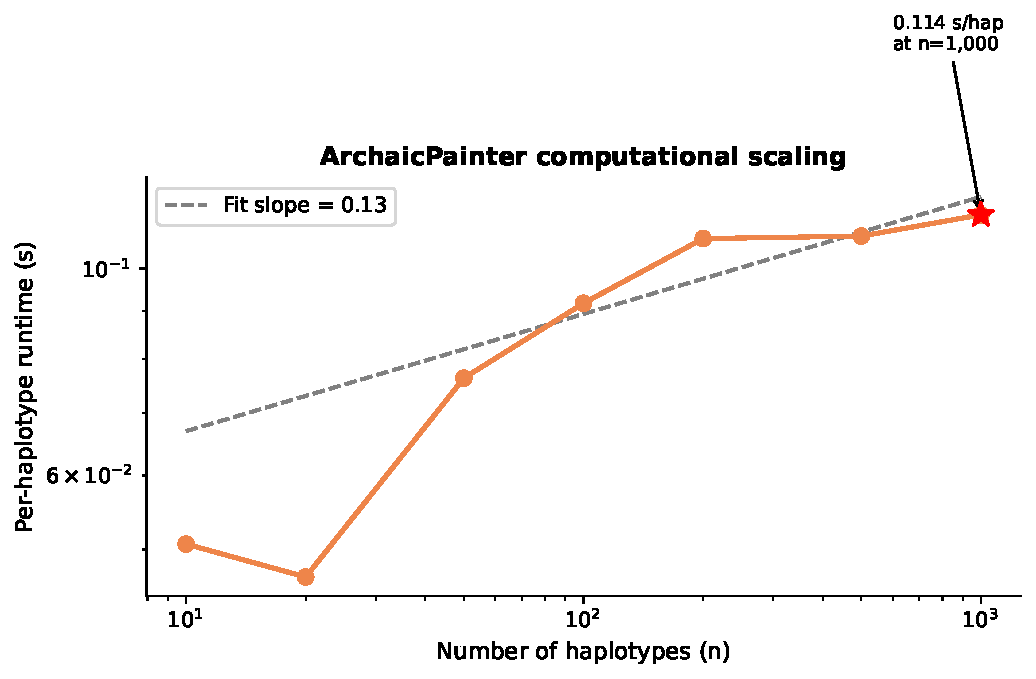
\includegraphics[width=0.65\textwidth]{figures/fig4_scalability}
\caption{\textbf{Near-linear computational scaling of ArchaicPainter.}
Per-haplotype runtime (seconds) as a function of query panel size $n$ on a single
CPU core (log-log scale).
Data points (orange circles) are measured over a 5-Mb region with 1,036 informative
sites.
The dashed grey line shows a log-log regression fit with empirical scaling exponent
$\approx 1.21$, close to the theoretical $O(n)$ for the Viterbi algorithm.
The red star marks $n = 1{,}000$ haplotypes (0.114~s/haplotype);
genome-wide extrapolation yields $\sim$19 cpu-hours (bp-based) or
$\sim$1 cpu-hour (site-density-based at 27 SNPs/Mb).}
\label{fig:scalability}
\end{figure}

%% ── Figure 5 ──────────────────────────────────────────────────────────────────
\begin{figure}[!ht]
\centering
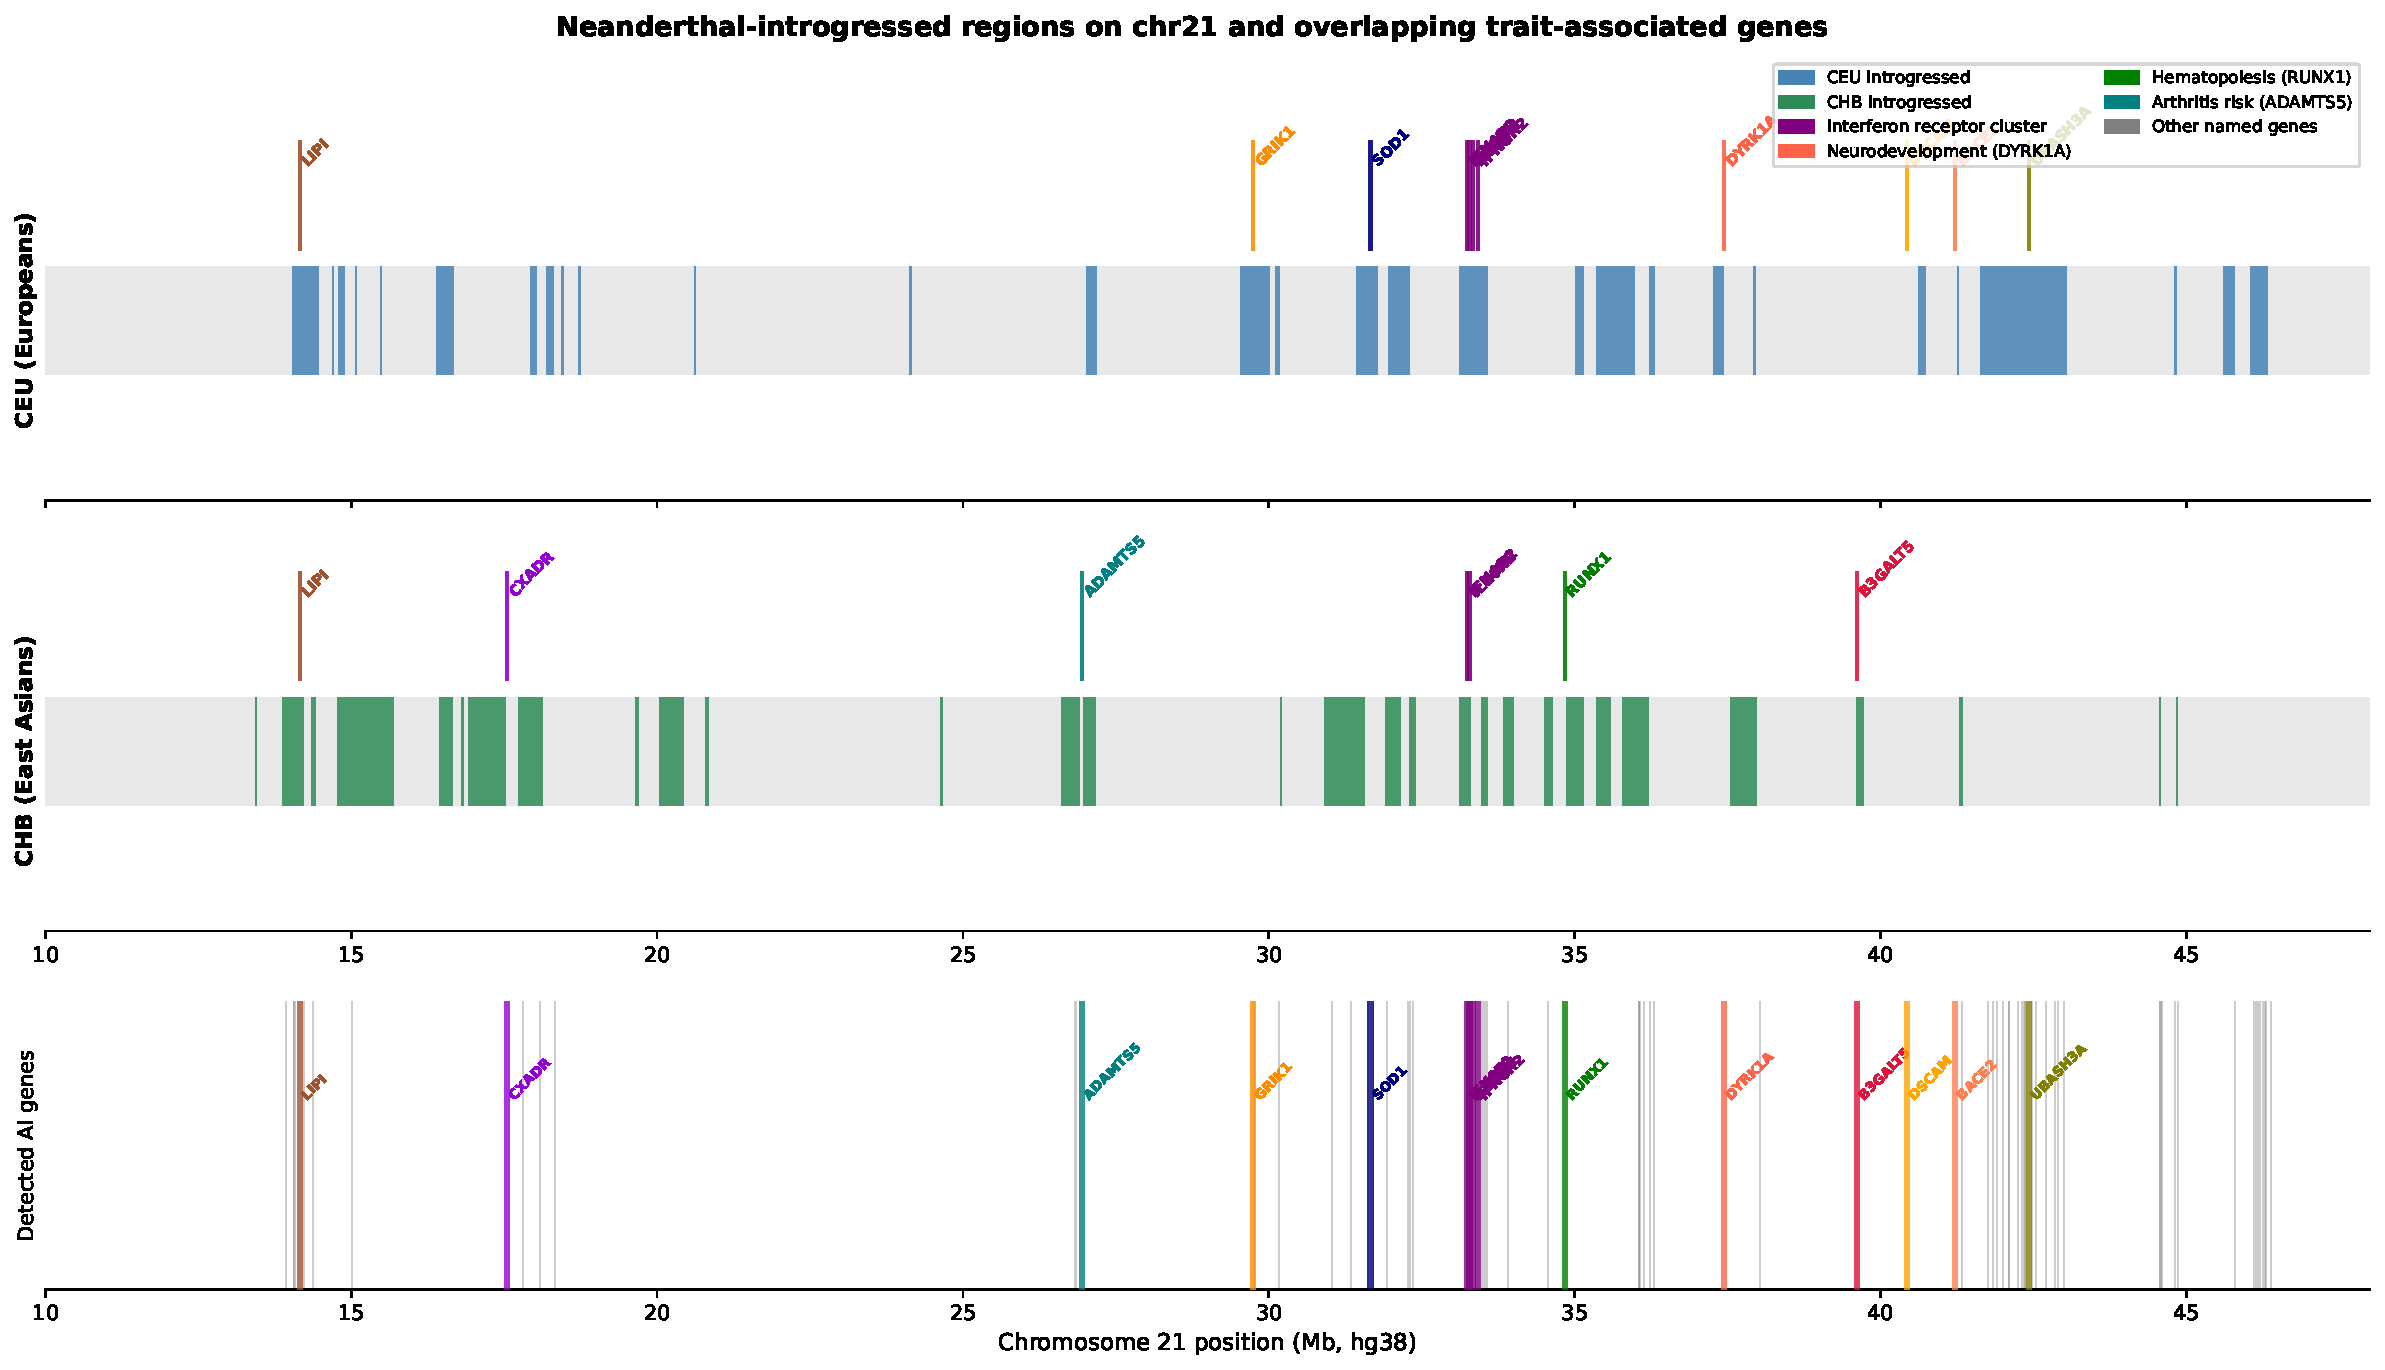
\includegraphics[width=\textwidth]{figures/fig5_functional_annotation}
\caption{\textbf{Functional annotation of ArchaicPainter-detected Neanderthal
introgressed regions on chromosome~21.}
Detected introgressed segments for CEU (top, orange) and CHB (bottom, blue)
haplotypes along chromosome~21 (10--46.7~Mb, GRCh38), with known trait-associated
genes annotated.
The complete type-I and type-II interferon receptor gene cluster
(\textit{IFNAR1}, \textit{IFNAR2}, \textit{IFNGR2}, \textit{IL10RB}) at
chr21:33.2--33.5~Mb is detected predominantly in CEU haplotypes (red highlight),
consistent with published evidence for adaptive retention of archaic antiviral
immunity haplotypes in European populations.
Population-specific signals include \textit{DYRK1A} (CEU; neurodevelopment) and
\textit{RUNX1}, \textit{ADAMTS5} (CHB; hematopoiesis, osteoarthritis).
In total, 7 of 16 previously published chr21 adaptive introgression candidates are
recovered among the 75 named genes overlapping \AP{}-detected regions
(Supplementary Table~S1).}
\label{fig:functional}
\end{figure}
